\documentclass[12pt]{article}
\usepackage{polski}
\usepackage[utf8]{inputenc}
\usepackage{amsfonts}
\usepackage{amsmath}
\usepackage{enumitem}
\usepackage{graphicx}
\setlength{\parskip}{1em}


\begin{document}
	\title{Sprawozdanie\\Metody Numeryczne 2, laboratorium 1}
	\author{Grzegorz Rozdzialik (D4, grupa lab. 2)}
	\maketitle	
	
	\section{Zadanie}
	{\Large Temat \textbf{2}, zadanie \textbf{49}:}\\
	Interpolacja funkcjami liniowymi na kwadracie podzielonym na $2n^2$ trójkątów przystających. Zagęszczanie podziału kwadratu, aż do osiągnięcia błędu średniokwadratowego, mierzonego w środkach ciężkości trójkątów, mniejszego od $\varepsilon$.
	
	\section{Opis metody}
	Mając funkcję interpolowaną $f: D \to \mathbb{R}$, gdzie $D = \{ (x, y) \in \mathbb{R}^2: x_0 \leq x \leq x_0 + H, y_0 \leq y \leq y_0 + H\}$, $H, x_0, y_0 \in \mathbb{R}$ opisaną na kwadracie o boku $H$, którego lewy dolny wierzchołek ma współrzędne $(x_0, y_0)$, należy skonstruować interpolującą funkcję sklejaną $p: D \to \mathbb{R}$ złożoną z funkcji opisanych na pojedynczych trójkątach przystających, dzielących ten kwadrat.
	
	\begin{figure}
		\centering
		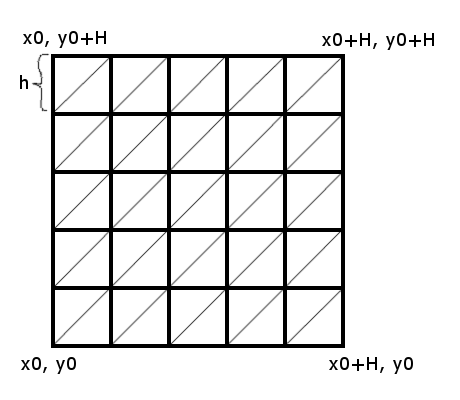
\includegraphics[scale=0.8]{square-division.png}
		\caption{Podział dziedziny funkcji $f$}
	\end{figure}
	
	Dziedzinę funkcji $f$ należy podzielić na $n$ części wzdłuż osi X oraz osi Y, co daje $n^2$ kwadratów, a następnie każdy kwadrat można podzielić względem dowolnej przekątnej na dwa trójkąty. W moim rozwiązaniu użyłem przekątnej o współczynniku kierunkowym równym $1$.
	
	\section{Implementacja metody}
	Przyjmijmy, że punkt $(x_0, y_0) \in D$ to lewy dolny wierzchołek dziedziny. Startując z parametrem $n = 1$ należy podzielić kwadrat na $n^2$ kwadratów przystających ($n$ podziałów wzdłuż osi X, $n$ podziałów wzdłuż osi Y), a następnie podzielić każdy z nich na dwa prostokątne trójkąty przystające, których przeciwprostokątną będzie przekątna kwadratu o współczynniku kierunkowym równym $1$.
	
	Niech $h = \frac{H}{n}$ będzie długością boku każdego z mniejszych kwadratów.
	
	Rozważmy jeden z kwadratów po podziale, będący w $i$-tym rzędzie i $j$-tej kolumnie. Wtedy jego lewy dolny wierzchołek ma współrzędne $(a, b) = (x_0 + (j-1)h, y_0 + (i-1)h)$.
	
	Wierzchołki trójkąta powyżej przekątnej kwadratu mają współrzędne $(a, b)$, $(a + h, b + h)$, $(a, b + h)$, a jego środek ciężkości znajduje się w punkcie $(a + \frac{h}{3}, b + \frac{2}{3}h)$.
	
	Wierzchołki trójkąta poniżej przekątnej kwadratu mają współrzędne $(a, b)$, $(a + h, b)$, $(a + h, b + h)$, a jego środek ciężkości znajduje się w punkcie $(a + \frac{2}{3}h, b + \frac{h}{3})$.
	
	Na rysunku 2 został przedstawiony podział kwadratu na dwa trójkąty przystające, oraz środek ciężkości jednego z trójkątów.
	
	\pagebreak
	
	\begin{figure}
		\centering
		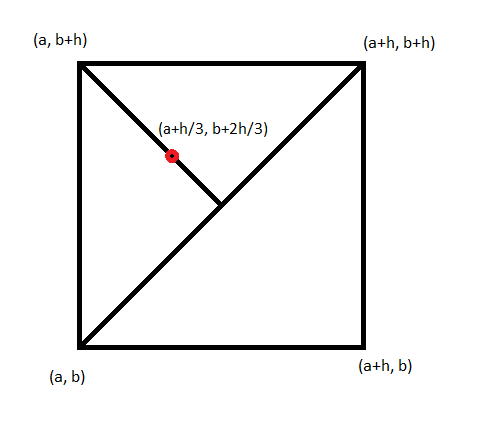
\includegraphics[scale=1]{images/single-square-gravity-center.png}
		\caption{Środek ciężkości trójkąta dzielącego kwadrat}
	\end{figure}
	
	Interpolacja będzie za pomocą funkcji liniowych, więc każda z funkcji $p$ ma równanie:
	$$p(x, y) = \alpha_0 + \alpha_1 x + \alpha_2 y$$
	gdzie $\alpha_0, \alpha_1, \alpha_2$ są współczynnikami specyficznymi dla danego trójkąta, na którym się odbywa interpolacja.
	
	Biorąc wierzchołki trójkątów za węzły interpolacji i korzystając z założenia, że dla węzłów interpolacji spełniony jest warunek:
	$$p(x_i, y_i) = f(x_i, y_i)$$
	gdzie $(x_i, y_i)$ są węzłami interpolacji, otrzymujemy następujący układ równań:
	\begin{align*}
		\left[
			\begin{array}{ccc}
				1 &  a  &  b  \\
				1 & a+h &  b  \\
				1 & a+h & b+h
			\end{array}
		\right]
		\left[
			\begin{array}{c}
				\alpha_0 \\
				\alpha_1 \\
				\alpha_2
			\end{array}
		\right]
		=		
		\left[
			\begin{array}{c}
				  f(a, b)   \\
				 f(a+h, b)  \\
				f(a+h, b+h)
			\end{array}
		\right]
	\end{align*}
	dla trójkąta powyżej przekątnej, oraz:
	\begin{align*}
		\left[
			\begin{array}{ccc}
				1 &  a  &  b  \\
				1 & a+h &  b  \\
				1 & a+h & b+h
			\end{array}
		\right]
		\left[
			\begin{array}{c}
				\alpha_0 \\
				\alpha_1 \\
				\alpha_2
			\end{array}
		\right]
		=		
		\left[
			\begin{array}{c}
				  f(a, b)   \\
				 f(a+h, b)  \\
				f(a+h, b+h)
			\end{array}
		\right]
	\end{align*}
	dla trójkąta poniżej przekątnej. Rozwiązując te układy równań otrzymujemy współczynniki potrzebne do wyznaczenia funkcji interpolującej $p$.
	
	\section{Warunek stopu}
	Podział zagęszczamy (zwiększamy parametr $n$), dopóki błąd średniokwadratowy mierzony w środkach ciężkości trójkątów jest większy od zadanej dokładności $\varepsilon$.
	
	Obliczenia kontynuujemy dopóki spełniony jest warunek:
	\begin{align*}
		\frac{\sum_{(x_j, y_i)} (f(x_j, y_i) - p(x_j, y_i))^2}{2n^2} \geq \varepsilon
	\end{align*}
	gdzie punkty $(x_j, y_i)$ są środkami ciężkości kolejnych trójkątów.
	
	\section{Poprawność metody}
	Metoda ta jest w ogólnym przypadku dość dokładna i spełnia założenia interpolacji (wartości w węzłach funkcji $p$ równe wartościom funkcji $f$).
	
	Mogą zdarzyć się przypadki funkcji, których wartości w środkach ciężkości trójkątów od razu będą bliskie wartościom dokładnym, przez co interpolacja się zakończy po pierwszym podziale, ale jest to wtedy wina warunku stopu, a nie samej metody. Niestety nie udało mi się znaleźć przykładu, który by to zobrazował.
	
	\section{Przykłady}
	\begin{enumerate}[label=\textbf{Przykład \arabic*}]
		\item
		Funkcja $f(x, y) = \sin{x} + \cos{y}$.\\
		Lewy dolny wierzchołek kwadratu: $(0, 0)$.\\
		Długość boku kwadratu: $2$.\\
		$\varepsilon = 10$
		
		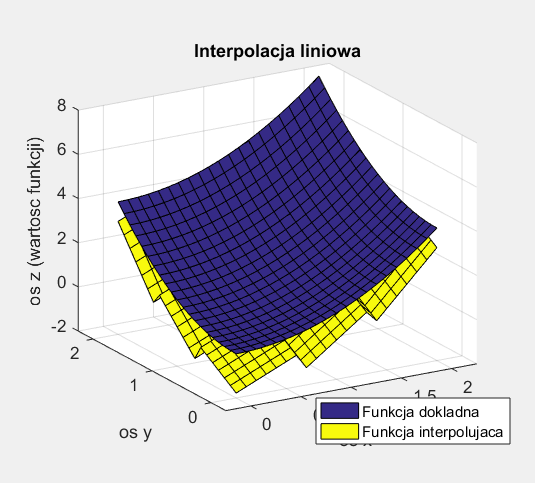
\includegraphics[]{images/example-1.png}
		
		\textbf{Wyniki}:\\
		Osiągnięto zadaną dokładność przy $n = 1$ ($2$ trójkątów przystających).\\
		Podział trwał $0.290355$ ms.\\
		Obliczanie ostatecznych współczynników dla funkcji interpolujących trwało $0.155429$ ms.\\
		Sprawdzanie ostatecznego błędu interpolacji trwało $0.061506$ ms.\\
		Osiągnięto błąd interpolacji równy $1.52815$ (zadano $10$).\\
		Obliczanie wartości do wykresu trwało $2.520103$ ms.
		\pagebreak
		
		
		\item
		Funkcja $f(x, y) = \sin{x} + \cos{y}$.\\
		Lewy dolny wierzchołek kwadratu: $(0, 0)$.\\
		Długość boku kwadratu: $2$.\\
		$\varepsilon = 1$
		
		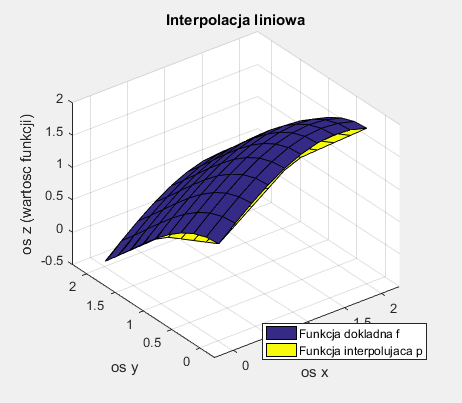
\includegraphics[]{images/example-2.png}
		
		\textbf{Wyniki}:\\
		Osiągnięto zadaną dokładność przy $n = 2$ ($8$ trójkątów przystających).\\
		Podział trwał $2.069056$ ms.\\
		Obliczanie ostatecznych współczynników dla funkcji interpolujących trwało $0.305593$ ms.\\
		Sprawdzanie ostatecznego błędu interpolacji trwało $0.181749$ ms.\\
		Osiągnięto błąd interpolacji równy $0.199071$ (zadano $1$).\\
		Obliczanie wartości do wykresu trwało $1.307705$ ms.
		\pagebreak
		
		
		\item
		Funkcja $f(x, y) = \sin{x} + \cos{y}$.\\
		Lewy dolny wierzchołek kwadratu: $(0, 0)$.\\
		Długość boku kwadratu: $2$.\\
		$\varepsilon = 0.1$
		
		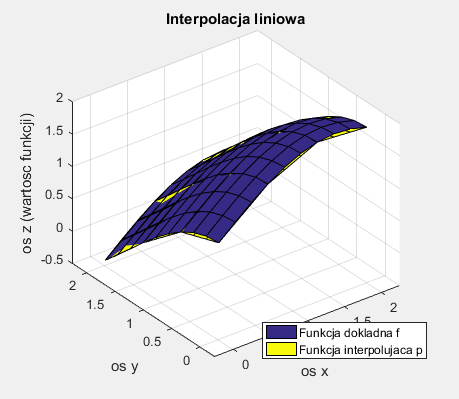
\includegraphics[]{images/example-3.png}
		
		\textbf{Wyniki}:\\
		Osiągnięto zadaną dokładność przy $n = 3$ ($18$ trójkątów przystających).\\
		Podział trwał $0.530563$ ms.\\
		Obliczanie ostatecznych współczynników dla funkcji interpolujących trwało $0.215273$ ms.\\
		Sprawdzanie ostatecznego błędu interpolacji trwało $0.025766$ ms.\\
		Osiągnięto błąd interpolacji równy $0.0446367$ (zadano $0.1$).\\
		Obliczanie wartości do wykresu trwało $0.212779$ ms.
		\pagebreak
		
		
		
		\item
		Funkcja $f(x, y) = \sin{x} + \cos{y}$.\\
		Lewy dolny wierzchołek kwadratu: $(0, 0)$.\\
		Długość boku kwadratu: $10$.\\
		$\varepsilon = 0.1$
		
		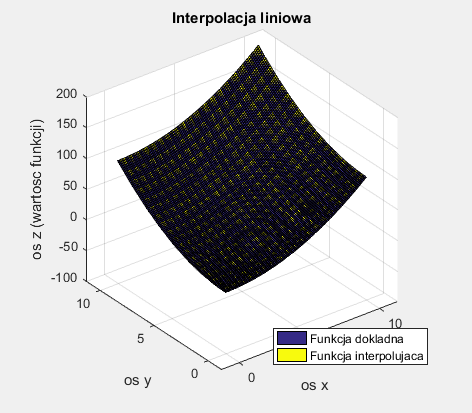
\includegraphics[]{images/example-4.png}
		
		\textbf{Wyniki}:\\
		Osiągnięto zadaną dokładność przy $n = 12$ ($288$ trójkątów przystających).\\
		Podział trwał $14.155078$ ms.\\
		Obliczanie ostatecznych współczynników dla funkcji interpolujących trwało $2.846198$ ms.\\
		Sprawdzanie ostatecznego błędu interpolacji trwało $0.210563$ ms.\\
		Osiągnięto błąd interpolacji równy $0.0778761$ (zadano $0.1$).\\
		Obliczanie wartości do wykresu trwało $0.280104$ ms.
		\pagebreak
		
		
		
		\item
		Funkcja: $f(x, y) = x^2 + y^2$.\\
		Lewy dolny wierzchołek kwadratu: $(0, 0)$.\\
		Długość boku kwadratu: $2$.\\
		$\varepsilon = 0.1$
		
		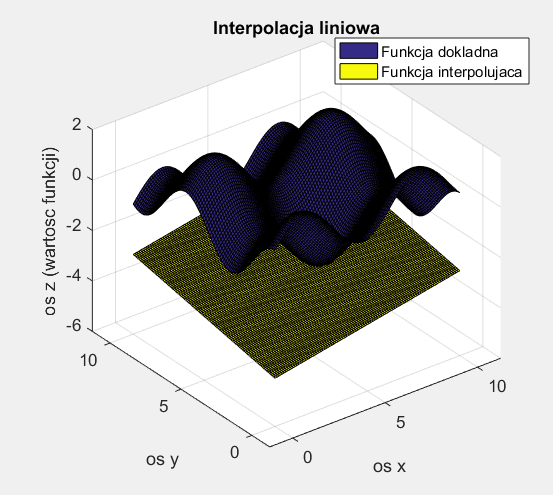
\includegraphics[]{images/example-5.png}
		
		\textbf{Wyniki}:\\
		Osiągnięto zadaną dokładność przy $n = 5$ ($50$ trójkątów przystających).\\
		Podział trwał $1.406614$ ms.\\
		Obliczanie ostatecznych współczynników dla funkcji interpolujących trwało $0.547463$ ms.\\
		Sprawdzanie ostatecznego błędu interpolacji trwało $0.037957$ ms.\\
		Osiągnięto błąd interpolacji równy $0.0619457$ (zadano $0.1$).\\
		Obliczanie wartości do wykresu trwało $0.243809$ ms.
		\pagebreak
		
		
		\item
		Funkcja: $f(x, y) = x^3 - y^2$.\\
		Lewy dolny wierzchołek kwadratu: $(0, 0)$.\\
		Długość boku kwadratu: $2$.\\
		$\varepsilon = 0.1$
		
		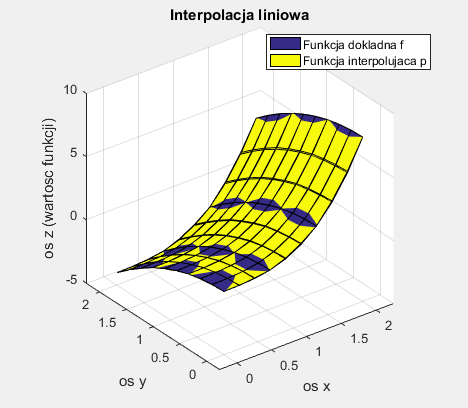
\includegraphics[]{images/example-6.png}
		
		\textbf{Wyniki}:\\
		Osiągnięto zadaną dokładność przy $n = 6$ ($72$ trójkątów przystających).\\
		Podział trwał $2.642008$ ms.\\
		Obliczanie ostatecznych współczynników dla funkcji interpolujących trwało $0.755809$ ms.\\
		Sprawdzanie ostatecznego błędu interpolacji trwało $0.065385$ ms.\\
		Osiągnięto błąd interpolacji równy $0.0946013$ (zadano $0.1$).\\
		Obliczanie wartości do wykresu trwało $0.144623$ ms.
		\pagebreak
		
		
		\item
		Funkcja: $f(x, y) = x^3 - y^2$.\\
		Lewy dolny wierzchołek kwadratu: $(0, 0)$.\\
		Długość boku kwadratu: $2$.\\
		$\varepsilon = 0.001$
		
		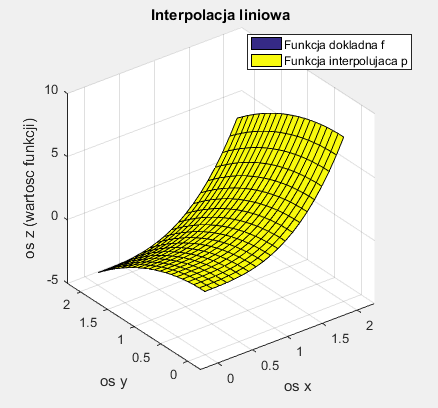
\includegraphics[]{images/example-7.png}
		
		\textbf{Wyniki}:\\
		Osiągnięto zadaną dokładność przy $n = 19$ ($722$ trójkątów przystających).\\
		Podział trwał $54.771794$ ms.\\
		Obliczanie ostatecznych współczynników dla funkcji interpolujących trwało $7.175479$ ms.\\
		Sprawdzanie ostatecznego błędu interpolacji trwało $0.567688$ ms.\\
		Osiągnięto błąd interpolacji równy $0.000829049$ (zadano $0.001$).\\
		Obliczanie wartości do wykresu trwało $0.313351$ ms.
	\end{enumerate}
	
	
	\section{Wnioski}
	\begin{enumerate}
		\item Wraz ze zmniejszaniem parametru $\varepsilon$ wykres funkcji interpolującej $p$ zbliża się do wykresu funkcji interpolowanej $f$ (przykłady 1, 2 oraz 3).

		\item Osiągnięcie dużej dokładności (poniżej $\varepsilon = 10^{-4}$) na dużym obszarze ($H \geq 10$) wymaga sporej ilości obliczeń.
		
		\item Interpolacja ta ma podobne wyniki do interpolacji z podziałem na $n^2$ kwadratów, ponieważ układy równań liniowych rozwiązywane dla każdego kwadratu okazują się być bardzo podobne.
	\end{enumerate}

	
	\section{Funkcja do testowania}
	Do sprawdzenia funkcji, które nie zostały udostępnione w interfejsie graficznym należy wykorzystać funkcję \textit{interpolateSquare}. Ta funkcja udostępnia funkcjonalność analogiczną do interfejsu graficznego.
	
	Więcej informacji dotyczących wykorzystania funkcji $interpolateSquare$ znajduje się w pliku z funkcją (\textit{interpolateSquare.m}).
	
	\section{Interfejs graficzny}
	Do metody został dodany interfejs graficzny, umożliwiający wygodne testowanie metody dla różnych parametrów i różnych funkcji interpolowanych $f$. Aby go wywołać należy uruchomić komendę \textit{interpolationGUI} w MATLABie.
	
	Został on przedstawiony na rysunku 3-cim.
	
	\begin{figure}
		\centering
		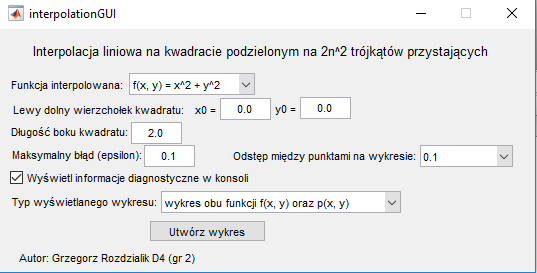
\includegraphics[scale=1]{images/gui.png}
		\caption{Interfejs graficzny}
	\end{figure}
	
	\pagebreak
	
	\section{Bibliografia}
	\begin{enumerate}
		\item P. Tatjewski \textit{Metody numeryczne}, Warszawa: Oficyna Wydawnicza PW, 2013
		\item Informacje z wykładu \textit{Metod numerycznych 2} (wydział MiNI PW, dr Iwona Wróbel)
	\end{enumerate}
	
\end{document}